One of the most important results of interest for this problem is how k-eff changes as the pin pitch is modified.  This result is shown below in figure \ref{f:keffVpitch}.  Out of the simulations that were run, the maximum k-effs are 1.07066 $\pm$ 0.00036 (track-length) and 1.07174 $\pm$ 0.00030 (collision), which both occurs at a pin pitch of 4.5 cm.

The shape of the curve is due to the fuel-to-moderator ratio.  At the smallest pin pitches, there is little moderator to slow down the neutrons, so they usually just get absorbed in the fuel instead of thermalizing and cuasing fission.  This effect would be mitigated some if fast fission in U-238 were considered in this model, but it is not.  For the largest pitches, there is a greater chance of neutrons being absorbed in the moderator, or simply never returning to the fuel after thermalizing.  Beginning at a pitch of 5.5 cm, this effect begins to dominate the benefits of moderation.

The reported uncertainty on the track-length estimator ranged from 31.4 pcm to 36.7 pcm.  For the collision estimator, they ranged from 27.2 pcm to 30.5 pcm.  \textbf{Is this what we expect?  I would have thought track length would be more consistent.}

\begin{figure}[H]
\centering
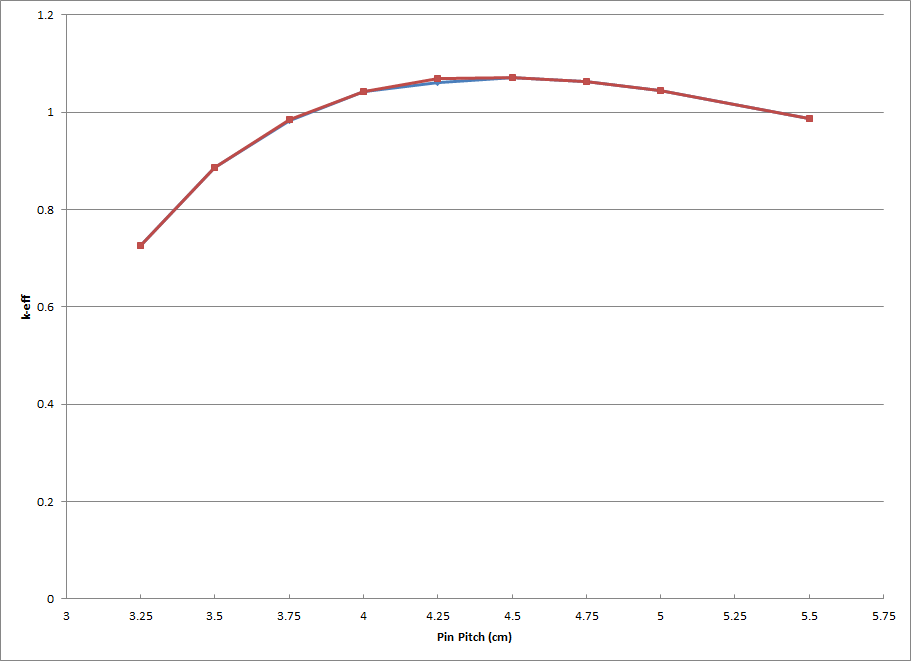
\includegraphics[width=0.8\linewidth]{images/keff_v_pitch.png}
\caption{Plot of track-length (blue) and collision (red) estimators of k-eff versus pin pitch}
\label{f:keffVpitch}
\end{figure}

A second quantity of interest is the leakage out of the pin cell, which is shown in figure \ref{f:leakVpitch}.  The leakage curves have some fluctuation in them, but generally have the same shape and similar magnitudes.  This is to be expected, since the problem is axially symmetric.  It also decreases with increasing pin pitch.  This occurs because the increase in the amount of moderator slows down the neutrons more effectively, which decreases their mean free path and reduces the probability of escaping the pin cell.

For both figures, error bars are included, but too small to be easily visible.  For figure \ref{f:keffVpitch}, this might be acceptable, but for figure \ref{f:leakVpitch} we would expect to see the two curves lying within each other's uncertainties.  However, in lecture it stated that the uncertainties which are reported are usually much lower than they should be.  This is due to the fact that all the neutrons in the active cycles are correlated to their predecessors, but uncertainty calculations assume completely independent samples.  Thus, this correlation makes the distributions appear more exact than they are.  This, combined with how relatively few scores occur on each of these estimators, explains why there is some discrepancy between the top and bottom leakages.

\begin{figure}[H]
\centering
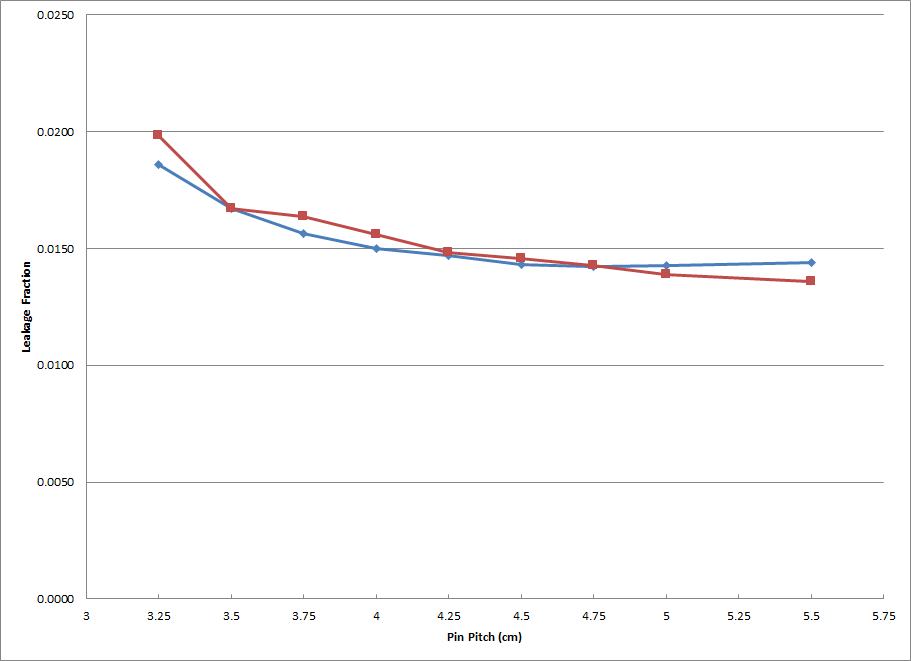
\includegraphics[width=0.8\linewidth]{images/leakage_v_pitch.png}
\caption{Plot of top (blue) and bottom (red) leakages versus pin pitch}
\label{f:leakVpitch}
\end{figure}